% !TEX TS-program = xelatex
\documentclass[FM]{tulpresentation}
\title{Tvorba a využití botu pro výuku matematiky na platformě Discord}
\author{Radek Mocek}
\institute{Ing. Igor Kopetschke}
\newcommand{\authorPhone}{}
\newcommand{\authorMail}{Aplikovaná informatika}
\setbeamertemplate{enumerate items}[default]
\newcommand{\h}[1]{{\usebeamercolor[fg]{framesubtitle}\textbf{#1}\par}}
\begin{document}
	\TULtitleframe
	
	\begin{frame}\frametitle{Cíle bakalářské práce}
		\begin{enumerate}
			\item Vypracujte rešerši sociálních platforem, které umožňují integraci botů.
			\item Analyzujte vybranou skupinu existujících botů na platformě Discord a knihoven pro jejich tvorbu.
			\item Navrhněte bot zaměřený na výklad a příklady z lineární algebry při využití specifických funkcí Discordu včetně administrace a interaktivních zpráv.
			\item Navržené řešení implementujte a nasaďte do testovacího provozu pro vybranou skupinu uživatelů.
			\item Vyhodnoťte zpětnou vazbu od uživatelů a navrhněte případné úpravy a vylepšení.
		\end{enumerate}
	\end{frame}
	
	\begin{frame}\frametitle{Navrhovaný výsledek bakalářské práce}
		\begin{itemize}
			\item Discord bot implementovaný v jazyce Python
			\begin{itemize}
				\item Knihovny discord.py, Matplotlib, NumPy, SymPy, UnicodeIt
			\end{itemize}
			\item Tři hlavní funkce v prostředí textového chatu
			\begin{itemize}
				\item Vykreslování matematických výrazů
				\item Výklad teorie
				\item Generace příkladů
			\end{itemize}
			\item Demonstrace specifických vlastností platformy Discord:			
		\end{itemize}
		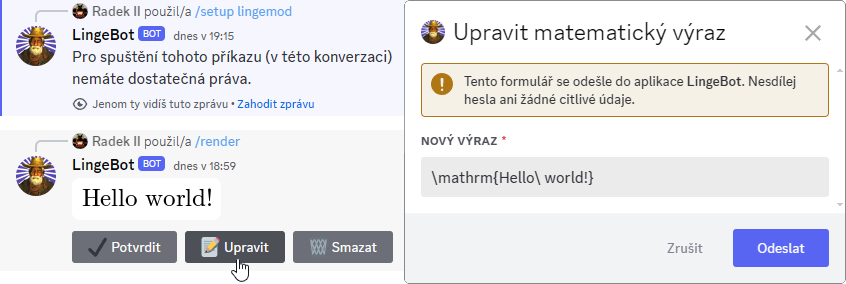
\includegraphics[width=.95\paperwidth]{img/idk}
	\end{frame}
	
	\begin{frame}\frametitle{Vykreslování matematických výrazů \texttt{/render}}
		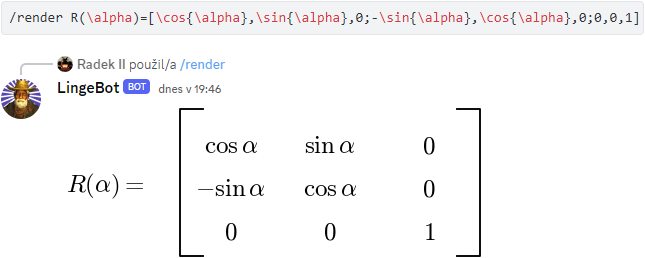
\includegraphics[width=.95\paperwidth]{img/idk2}
		\begin{itemize}
			\item Matplotlib Mathtext vs TeX
			\item Vykreslování matic a jejich zápis
			\item Rovnice s maticemi a aproximace délky výrazu
		\end{itemize}
	\end{frame}
	
	\begin{frame}\frametitle{Výklad teorie \texttt{/explain}}
		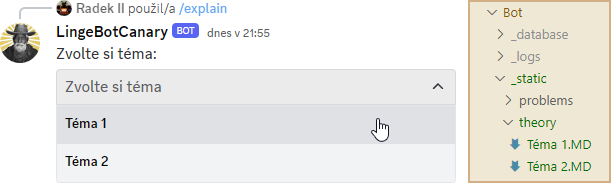
\includegraphics[width=.95\paperwidth]{img/idk3}
		\begin{itemize}
			\item Čtení z Markdown souborů
			\item ,,Hot reload``
			\item \texttt{\$\$\$render} $\to$ \texttt{/render}
			\item \texttt{<sub>} a \texttt{<sup>} $\to$ Unicode
			\item Obrázky přes internetový odkaz
		\end{itemize}
	\end{frame}
	
	\begin{frame}[plain]
		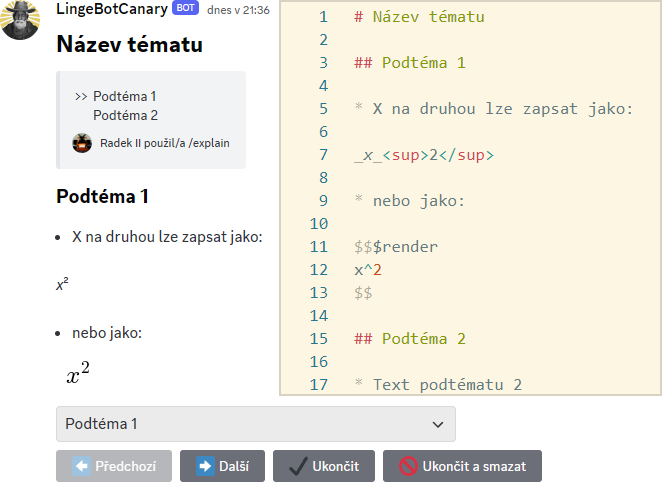
\includegraphics[width=.95\paperwidth]{img/idk4}
	\end{frame}
	
	\begin{frame}\frametitle{Generování příkladů \texttt{/generate}}
		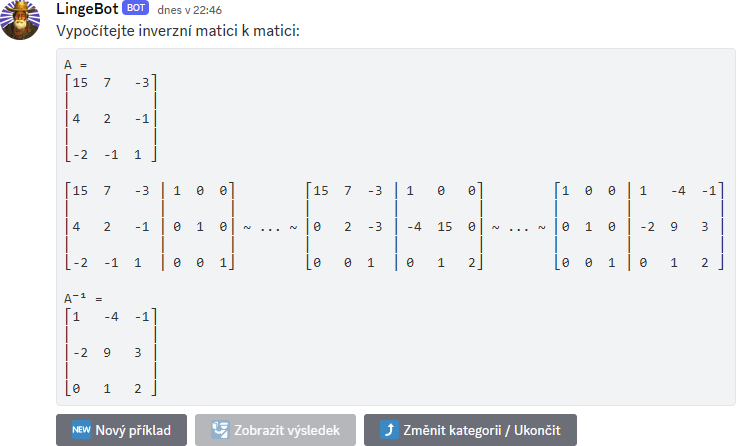
\includegraphics[width=.95\paperwidth]{img/idk5}
	\end{frame}
	
	\begin{frame}[plain]\frametitle{Diagram tříd generátoru příkladů}
		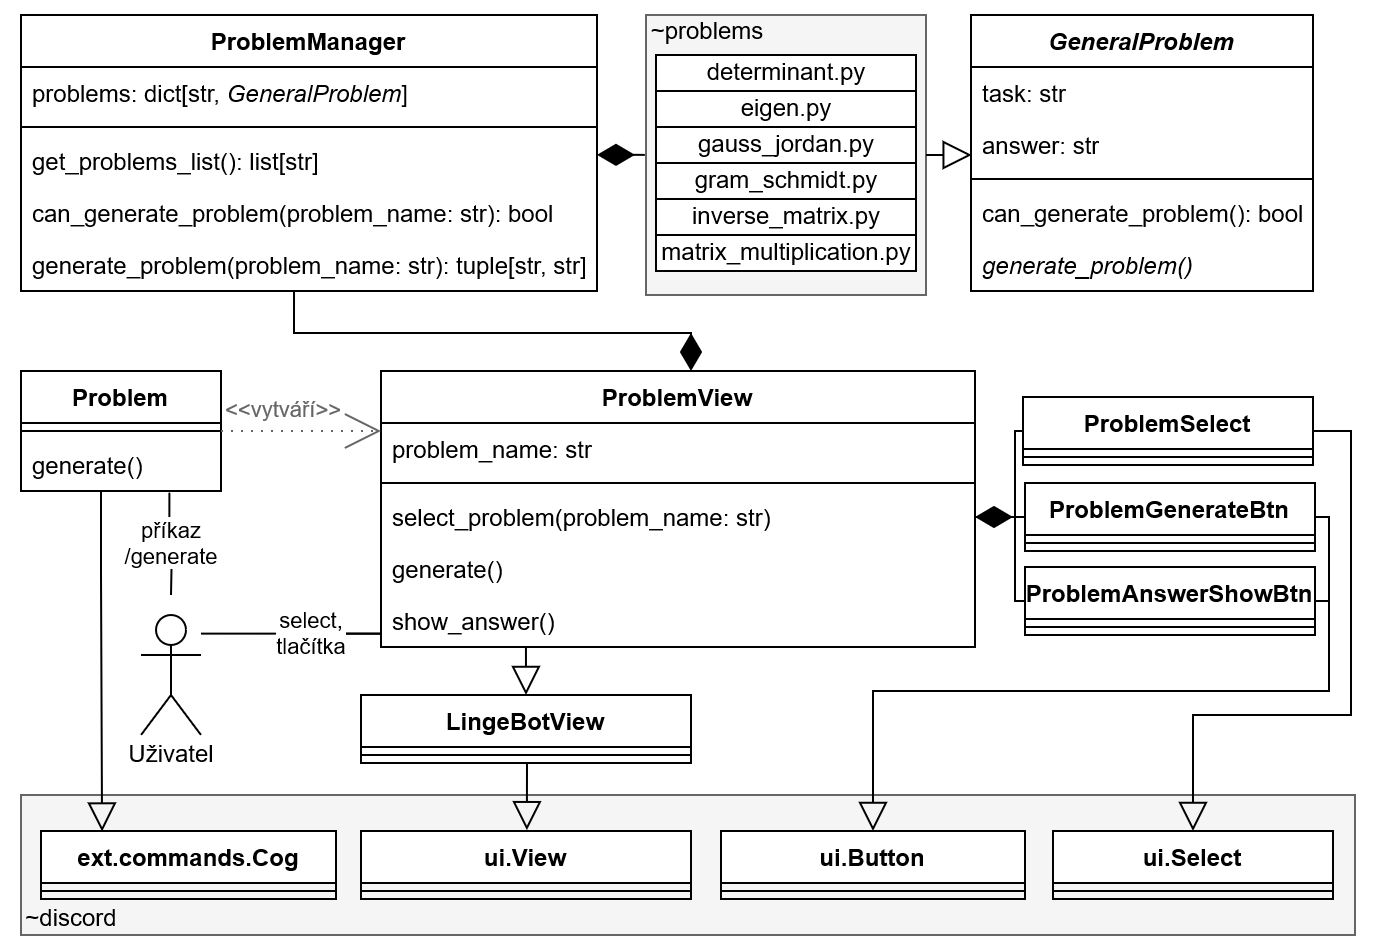
\includegraphics[width=.95\paperwidth]{img/idk6}
	\end{frame}
	
	\begin{frame}[plain]\frametitle{Sada příkazů \texttt{/setup}}
		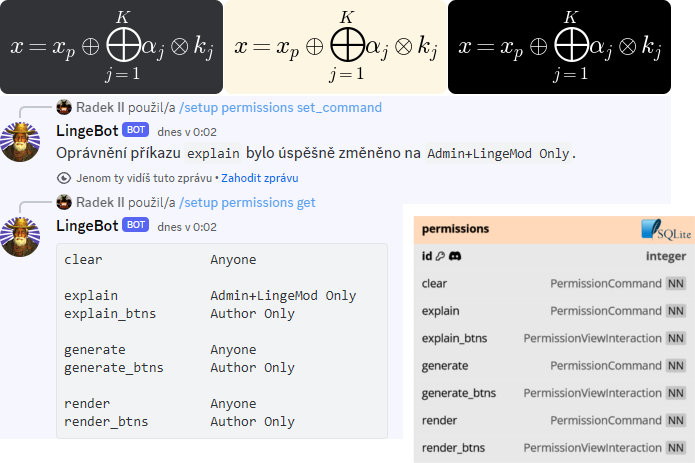
\includegraphics[width=.95\paperwidth]{img/idk7}
	\end{frame}
	
	\begin{frame}\frametitle{Závěr}
		\h{Shrnutí}
		\begin{itemize}
			\item Rešerše sociálních platforem podporujících boty
			\item Rešerše matematiky a knihoven pro tvorbu botů na Discordu
			\item Funkční bot
			\begin{itemize}
				\item \texttt{/render}, \texttt{/explain}, \texttt{/generate}
				\item Interaktivní prvky a oprávnění
				\item SQLite
				\item Možnost self-host, důraz na rozšiřitelnost
			\end{itemize}
			\item Ukázkové materiály
		\end{itemize}
		\h{Možná vylepšení}
		\begin{itemize}
			\item \texttt{/render} – obrázky ze souboru a vyhledávání
			\item \texttt{/generate} – generovat sadu různých příkladů
			\item Lepší aproximace délky výrazu (\texttt{\textbackslash alpha} $\to$ 1, \texttt{\textbackslash sin} $\to$ 3, \dots)
			\item Použít SQLAlchemy
		\end{itemize}
	\end{frame}
	
	\TULendframe
\end{document}
